\documentclass[a4paper]{report}

%====================== PACKAGES ======================

\usepackage[french]{babel}
%pour gérer les positionnement d'images
\usepackage{float}
\usepackage{amsmath}
\usepackage{graphicx}
\usepackage[colorinlistoftodos]{todonotes}
\usepackage{url}
%pour les informations sur un document compilé en PDF et les liens externes / internes
\usepackage{hyperref}
%pour la mise en page des tableaux
\usepackage{array}
\usepackage{tabularx}
%pour utiliser \floatbarrier
%\usepackage{placeins}
%\usepackage{floatrow}
%espacement entre les lignes
\usepackage{setspace}
%modifier la mise en page de l'abstract
\usepackage{abstract}
%police et mise en page (marges) du document
\usepackage[T1]{fontenc}
\usepackage[top=2cm, bottom=2cm, left=2cm, right=2cm]{geometry}
%Pour les galerie d'images
\usepackage{subfig}
\usepackage{amsthm,thmtools}
\usepackage{xcolor}
\usepackage{framed}
\colorlet{shadecolor}{lightgray!25}
%====================== INFORMATION ET REGLES ======================

%rajouter les numérotation pour les \paragraphe et \subparagraphe
\setcounter{secnumdepth}{4}
\setcounter{tocdepth}{4}

\hypersetup{							% Information sur le document
pdfauthor = {Premier Auteur},			% Auteurs
pdftitle = {Nom du Projet -
			Sujet du Projet},			% Titre du document
pdfsubject = {Rapport de Stage},		% Sujet
pdfkeywords = {Tag1, Tag2, Tag3, ...},	% Mots-clefs
pdfstartview={FitH}}					% ajuste la page à la largueur de l'écran
%pdfcreator = {MikTeX},% Logiciel qui a crée le document
%pdfproducer = {}} % Société avec produit le logiciel

\newcommand{\cmark}{\ding{51}}%
\newcommand{\xmark}{\ding{55}}%

\newtheorem{post}{Postulat}
\newtheorem{mydef}{Définition}
%%
%======================== DEBUT DU DOCUMENT ========================

\begin{document}

%régler l'espacement entre les lignes
\newcommand{\HRule}{\rule{\linewidth}{0.5mm}}

%page de garde
\begin{titlepage}
\begin{center}

% Upper part of the page. The '~' is needed because only works if a paragraph has started.

\includegraphics[width=0.35\textwidth]{./logo}~\\[1cm]

\textsc{\LARGE Université de Reims Champagne Ardennes}\\[1.5cm]

\textsc{\Large }\\[0.5cm]

% Title
\HRule \\[0.4cm]

{\huge \bfseries  
Mise en place d'une solution d'évaluation des performances de solutions de virtualisation, basée sur une expérience utilisateur\\[0.4cm] }

\HRule \\[1.5cm]

% Author and supervisor
\begin{minipage}{0.4\textwidth}
\begin{flushleft} \large
\emph{Auteur:}\\
HERARD \textsc{Joffrey}\\
\end{flushleft}
\end{minipage}
\begin{minipage}{0.4\textwidth}
\begin{flushright} \large
\emph{Responsable:} \\
Olivier \textsc{FLAUZAC}\\
\end{flushright}
\end{minipage}

\vfill

% Bottom of the page
{\large \today}

\end{center}
\end{titlepage}


%page blanche
\newpage
~
%ne pas numéroter cette page
\thispagestyle{empty}
\newpage

\renewcommand{\abstractnamefont}{\normalfont\Large\bfseries}
%\renewcommand{\abstracttextfont}{\normalfont\Huge}

\begin{abstract}
\hskip7mm

\begin{spacing}{1.3}
L'objet de notre étude a porté sur l'ensemble des solutions de virtualisation disponibles et possibles dans le cadre de la machine support mise à disposition. Il semble essentiel de rappeler que ces solutions sont variées dans leur fondamentalisme, leurs principes ou bien encore dans leurs domaines traditionnels d'utilisation. Afin de mettre en place une solution d'évaluation des solutions de virtualisation du point de vue des utilisateurs nous avons défini des scénarios de tests et des domaines d'études spécifiques de test sur chaque composant du système qui pourrait être utilisés par un ensemble d'utilisateurs. Pour cela, il a fallut définir ce qui allait être étudié sur chaque composant mais aussi comment mettre en oeuvre ces tests sur l'ensemble de ces machines. Je pus alors me poser un certain nombre de questions : Quels outils existent ? Comment faire la mise en place de ces outils ? Comment faire l'analyse de l'ensemble des résultats ? Comment faire l'établissement des liens et d'une échelle de performances ? Comment faire pour délimiter les meilleurs domaines de chaque solutions de virtualisation ?
\end{spacing}
\end{abstract}


\tableofcontents
\thispagestyle{empty}
\setcounter{page}{0}
%ne pas numéroter le sommaire

\newpage

%espacement entre les lignes d'un tableau
\renewcommand{\arraystretch}{1.5}

%====================== INCLUSION DES PARTIES ======================

~
\thispagestyle{empty}
%recommencer la numérotation des pages à "1"
\setcounter{page}{0}
\newpage

	   
\chapter{Présentation du projet}

Durant cette présentation du projet, il seras présenté l'ensemble du sujet, sur les différents termes employé, des choix qui on été fait sur certaines technologies, la problématiques soulevé par le sujet. Les solutions émient pour résoudre les différentes problématiques qui sont levées. 
%note en bas de page

\section{Sujet}

La mise en place d'une solution d’évaluation des performances de solutions de virtualisation, basée sur une expérience utilisateur, est donc le sujet de ce stage, plusieurs termes on été définis. Ceux ci on été déterminer durant ce stage pour cerner ce dont-il était vraiment question.  On va d'abord définir les termes qui sont intéressant à développé comme, solutions de virtualisation, évaluation de ces solutions, expérience utilisateurs. 
Tout d'abord les solutions de virtualisation c'est quoi ? 

\begin{mydef}
Solutions de virtualisation : La virtualisation consiste à faire fonctionner un ou plusieurs systèmes d'exploitation / applications comme un simple logiciel, sur un ou plusieurs ordinateurs. Actuellement sépare en deux grand domaine, l’hyper-vision(eux meme divisé en deux type : Type 1 et type 2) et la conteneurisation.
\end{mydef}

Finalement une fois les termes des solution de virtualisation définie en détails, il est nécessaires de donner une définition de ce que c'est de faire une évaluation des performances. 
\newpage
\section{Objectifs}
\begin{enumerate}
	\item Savoir évaluer les différentes solutions de virtualisation. 	
	\item Effectuer une démarche scientifique cohérente.
	\item Effectuer un travail collaboratif avec des personnes d’expériences sur le sujet, qui malgré tout est plus ou moins inédit pour moi (J’entends que la plupart des travaux réalisé ces dernières années on été fait avec des gens de mêmes expérience que moi ).
	\item Établir des statistiques, sur les résultats qui seront obtenus . En ressortir des résultats des variables qui sortent du lot.
	\item Établir un tableau récapitulatif afin de pouvoir résumé toutes les données obtenus .
	
\end{enumerate}
\section{Problématique soulevée}

\begin{center} 
Comment mettre en œuvre des scénarios afin d'évaluer de manière efficace et juste sans interférer dans les résultats, les différentes solutions de virtualisation et de conteneurisation sur le plan du HDD, CPU, GPU, Réseaux ? 
\end{center}

\section{Hypothèse de solution}

%Quoi :
Il existe un ensemble de logiciel type pour le provisionning de machine virtuelle, ainsi que d'outils afin de benchmark qui sont neutre dans leur prise de ressource.

\chapter{Analyse de l'existant}

Dans ce chapitre, nous verrons quelles technologies existent pour répondre à notre problématique.

\section{Virtualisation}



\subsection{Hyperviseurs}
\begin{mydef}
Hyperviseurs : C'est une plate-forme de virtualisation qui permet à plusieurs systèmes d'exploitation de travailler sur une même machine physique en même temps. Il en existe deux catégories : 
	\begin{itemize}
		\item La première bien nommée Type 1 : est un logiciel de virtualisation installé directement sur le matériel informatique, il contrôle non seulement le matériel, mais aussi un ou plusieurs systèmes d'exploitation invités.
		\item La deuxième bien nommée Type 2 : sont des applications de virtualisation qui s’exécutent non pas directement sur du hardware mais sur un système d’exploitation.
	\end{itemize}
\end{mydef}
Il existe un ensemble d'Hyperviseur de type 1, que l'on peut lister de manière non exhaustive : 

\begin{itemize}
\item CP
\item XEN
\item ESX Server
\item LPAR
\item Hyper-V
\item Proxmox
\item KVM
\end{itemize}

Il existe un ensemble d'Hyperviseur de type 2, que l'on peut lister de manière non exhaustive : 

\begin{itemize}
\item VMWare Server
\item VMWARE Workstation
\item QEMU
\item Hyper-V
\item Parallels Workstation
\item Parallels Dekstop
\item VirtualBox
\end{itemize}
\subsection{Conteneurs}

\begin{mydef}
Conteneurs : C'est de créer des instances dans un espace isolé au lieu. En d'autres termes, le partage du matériel est de rendre disponible de nombreux opérateurs sur le noyau lui-même plutôt que d'une autre couche. 
\end{mydef}

Il existe un ensemble de gestion de conteneurs, que l'on peut lister de manière non exhaustive : 
\begin{itemize}

\item LXC
\item Docker
\end{itemize}
\section{Provisionning}
 
\begin{mydef}
Provisionning : C'est l'approvisionnement de machines, afin de mettre en place des configurations, des allocations automatiques de ressources, voir même des installations de logiciel, gestions de configuration, maintenance système. Globalement il sert à faire de la gestion de groupe de machines. 
\end{mydef}
Initialement le provisioning était du scripting manuel, voir même des solutions Client/Serveur, avec un serveur de configuration et un ensemble d'agents de gestion placés sur les machines à administrer. On appelle cela un framework d’exécution distantes depuis une station de gestion.
Le scripting a malgré tout des limites, cela représente un travail fastidieux, il fait souvent face à un problème d'hétérogénéité. On peut se retrouver face un script spécifique pour une opération, par serveur, par service.
Voici une liste :
\begin{itemize}

\item Ansible
\item Vagrant
\item Saltstack
\item Libvirt
\end{itemize}
\section{Benchmarking}
Une évaluation des performances est appelée souvent dans le monde anglophone un Benchmark. Ce terme est défini comme suit.
\begin{mydef}
Benchmarking : Évaluation des performances d'un système par simulation des conditions réelles d'utilisations. 
\end{mydef}
Il existe un certain nombre de benchmark référence en majeur partie par OpenBenchmark.com, les sources de ces benchmark sont réalisées avec le célèbre outil nommé Phoronix tests suite.


 
\chapter{Analyse des besoins}

Intro

\section{Plan d'expériences}

Après une analyse des besoins fonctionnels du projet, nous avons défini deux sous catégories. D'un côté, les besoins [...], de l'autre, les besoins [...].

\subsection{Expérimentation disque dur}

Bla

\subsection{Expérimentation processeur}

Bla

\subsection{Expérimentation carte graphique}

Bla
\subsection{Expérimentation réseaux}

Bla
\newpage

\section{Choix sur les outils de virtualisation}

Comme précédemment, nous avons choisi de distinguer deux catégories pour les besoins non-fonctionnels. D'une part, nous avons les besoins non-fonctionnels pour les [...], et d'autre part ceux pour [...]. Nous avons aussi pris en compte les contraintes de développement, que nous détaillerons à la fin de cette partie.

\subsection{Hyperviseurs}

Bla\\


\newpage
\subsection{Conteneurs}

Bla\\


\newpage

\section{Choix d'outils d’évaluation}

Intro

\subsection{Outils d'évaluation personnel}

Bla\\

\subsection{Phoronix}

Bla\\

\section{Choix d'outils d'orchestration}

Intro

Bla\\
\subsection{Saltstack}

Bla\\

\subsection{Phoromatic}

Bla\\

\subsection{Libvirt}

Bla\\

\chapter{Résultats}

\section{Partie processeurs}

Intro

\subsection{Scénario 1 : bla bla }

\paragraph*{Paragraphe 1 (n'apparaitra pas dans l'index)} Bla

\paragraph*{Paragraphe 2} Bla

\paragraph*{Paragraphe 3} Bla

\subsection{Scénario 2 : bla bla }

Bla

\subsection{Scénario 3 : bla bla }

Bla

\section{Partie Disque dur }

Intro
Partie

\subsection{Scénario 1 : bla bla }

\paragraph*{Paragraphe 1 ('apparaitra pas dans l'index)} Bla

\paragraph*{Paragraphe 2} Bla

\paragraph*{Paragraphe 3} Bla

\newpage

\subsection{Scénario 2 : bla bla }


\subsection{Scénario 3 : bla bla }


\section{Partie Réseaux }

Intro
Partie

\subsection{Scénario 1 : bla bla }

\paragraph*{Paragraphe 1 ('apparaitra pas dans l'index)} Bla

\paragraph*{Paragraphe 2} Bla

\paragraph*{Paragraphe 3} Bla

\newpage

\subsection{Scénario 2 : bla bla }


\subsection{Scénario 3 : bla bla }



\section{Partie d'utilisation différentes}

Intro
Partie

\subsection{Scénario 1 : bla bla }

\paragraph*{Paragraphe 1 ('apparaitra pas dans l'index)} Bla

\paragraph*{Paragraphe 2} Bla

\paragraph*{Paragraphe 3} Bla

\newpage

\subsection{Scénario 2 : bla bla }


\subsection{Scénario 3 : bla bla }



\newpage

\chapter{Bilan}

%Rappel du context
Intro / Rappel Contexte

Nous avons donc pu en tirer la problématique suivante :

\begin{center}
\hskip7mm
Problématique du sujet
\end{center}


%Rappel des résultats
Bla

\newpage

%Conclusion/Perspectives


\newpage
\section{Annexes}
%Ne pas numéroter cette partie
\part*{Annexes}
%Rajouter la ligne "Annexes" dans le sommaire
\addcontentsline{toc}{part}{Annexes}

\chapter*{Annexe 1}
\addcontentsline{toc}{chapter}{Annexe 1}

%changer le format des sections, subsections pour apparaittre sans le num de chapitre
\makeatletter
\renewcommand{\thesection}{\@arabic\c@section}
\makeatother

%recommencer la numérotation des section à "1"
\setcounter{section}{0}

Intro

\section{Partie 1}

Bla

\subsection{Sous-partie 1}

Bla

\subsection{Sous-partie 2}

Bla

\subsection{Sous-partie 3}

Bla

\section{Partie 2}

Bla

\subsection{Sous-partie 1}

Bla

\subsection{Sous-partie 2}

Bla

\subsection{Sous-partie 3}

Bla

\chapter*{Annexe 2}
\addcontentsline{toc}{chapter}{Annexe 2}

%recommencer la numérotation des section à "1"
\setcounter{section}{0}

Intro

\section*{Prérequis}
\addcontentsline{toc}{section}{Prérequis}

Bla

\begin{itemize}
\item item1;
\item item2;
\item item3;
\item item4.
\end{itemize}

Bla

\section{Partie 1}

Bla

\subsection{Sous-parie 1}

Bla

\subsection{Sous-parie 2}

Bla

\section{Partie 2}

\begin{center}
\textsc{Attention !}

\textit{Texte d'avertissement}
\end{center}

Bla

\newpage

\section{Partie 3}

Bla

\begin{figure}[!ht]
\begin{center}
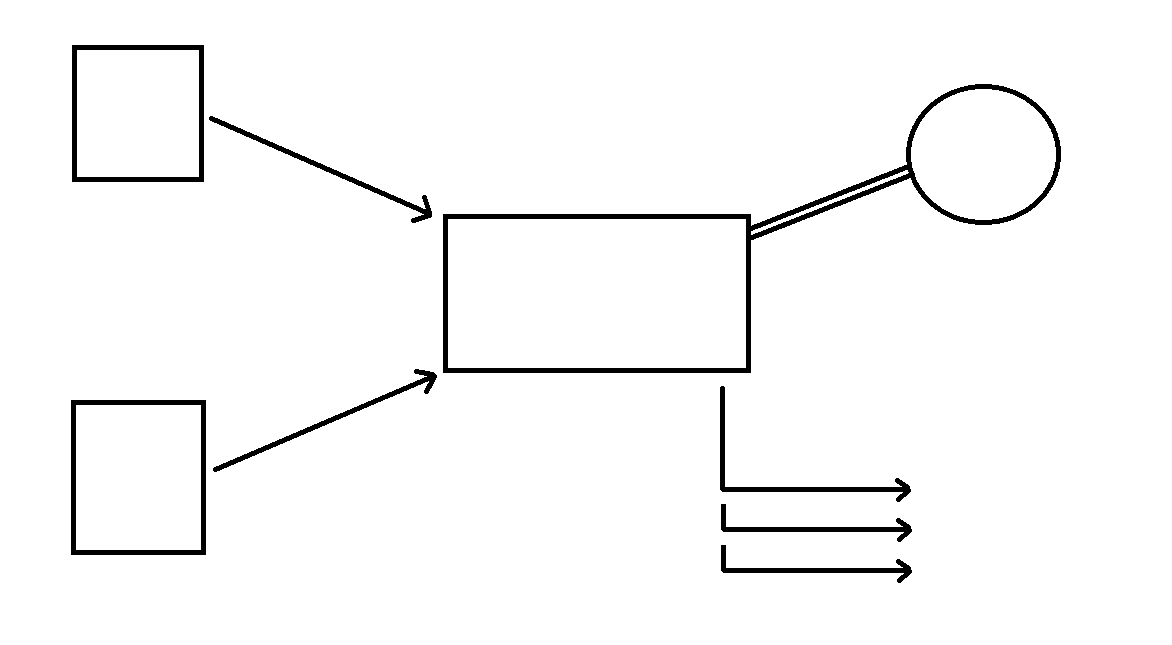
\includegraphics[height=8cm]{presentation/schema}
\end{center}
\caption[schema]{Presentation schema}
\end{figure}

\paragraph*{Paragraphe 1}
~\\
\hskip7mm

Bla

\paragraph*{Paragraphe 2}
~\\
\hskip7mm

Bla

\paragraph*{Paragraphe 3}
~\\
\hskip7mm

Bla

\newpage
\begin{thebibliography}{9}

   \bibitem{Docker}
          Documentation Docker
          \url{https://docs.docker.com/}.
   \bibitem{HyperV Conteneurs}
          Hyper-V Containers
          \url{https://docs.microsoft.com/en-us/virtualization/windowscontainers}.
   \bibitem{Linux containers}
         Linux Containers
         \url{https://linuxcontainers.org/fr/}.
   \bibitem{Virtual Box}
         Virtual Box
         \url{ https://www.virtualbox.org/}.
   \bibitem{Proxmox VE}
         Proxmox VE
         \url{https://www.proxmox.com/en/}.
   \bibitem{VmWare}
         VmWare
         \url{ http://www.vmware.com/fr.html}.
   \bibitem{QEMU}
         QEMU
         \url{http://www.qemu-project.org/   }.
   \bibitem{Hyper-V}
         Hyper-V
         \url{https://www.microsoft.com/fr-fr/cloud-platform/server-virtualization}.      
   \bibitem{KVM}
         KVM
         \url{https://www.linux-kvm.org/}.
   \bibitem{VMMark}
         VM Mark
         \url{https://www.vmmark.com/products/vmark.html}. 
   \bibitem{VM history}
         VM history par IBM
         \url{http://www.vm.ibm.com/history/ }.
 
   \bibitem{Art1}
          An Analysis of Performance Interference Effects in Virtual Environments
          \url{http://ieeexplore.ieee.org/document/4211036/?arnumber=4211036}
      
   \bibitem{Art2}
          The impact of Docker containers on the performance of genomic pipelines
          \url {https://www.ncbi.nlm.nih.gov/pmc/articles/PMC4586803/}              
   \bibitem{Art3}
          \url{Wei Huang, Jiuxing Liu, Bulent Abali et Dhabaleswar K. Panda, « A Case for High Performance Computing with Virtual Machines », ICS '06, ACM, série ICS '06,‎ 2006, p. 125–134 (ISBN 1-59593-282-8, DOI 10.1145/1183401.1183421}      
          \bibitem{Art4}
          \url{Piotr Luszczek, Eric Meek, Shirley Moore et Dan Terpstra, Evaluation of the HPC Challenge Benchmarks in Virtualized environments, Springer Berlin Heidelberg, coll. « Lecture Notes in Computer Science », 29 août 2011 }
   \bibitem{Documentation de PTS}
         GitHub documentation de Phoronix test suite.
          \url{https://gist.github.com/anshula/728a76297e4a4ee7688d#the-easy-way}.
          
   \bibitem{Site de SaltStack}
        Site officiel de SaltStack
          \url{https://saltstack.com/}.

   \bibitem{Documentation de SaltStack}
         Documentation de SaltStack.
          \url{https://docs.saltstack.com/en/latest/}.
          
   \bibitem{Documentation de SaltStack2}
       
          \url{https://docs.saltstack.com/en/latest/topics/installation/debian.html}.

   \bibitem{Documentation de Phoromatic}
       
          \url{https://www.phoronix-test-suite.com/documentation/phoromatic.html}.
\end{thebibliography}


\end{document}